\chapter{Was ist ein DDoS-Angriff?}
\label{chap:kapitel1}

Die Grundlage für einen \ac{ddos}-Angriff ist ein \ac{dos}-Angriff. Ein \ac{dos}-Angriff (Denial-of-Service-Angriff) hat das Ziel ein System nicht mehr verfügbar zu machen. Dazu kann entweder die begrenzte Bandbreite so ausgenutzt werden, dass die eigentlichen Nutzer des Systems dieses nicht mehr erreichen können. Eine andere Möglichkeit ist die Überlastung des Systems selbst (CPU, RAM, ...), damit dieses nicht mehr (zeitnah) antworten kann.

Eine Analogie zu einem DoS-Angriff aus dem realen Leben wäre die Benutzung von einem Bus. Spricht man sich hierbei ab, dass sehr viele Leute gleichzeitig versuchen in einen Bus einzusteigen, so bleibt kaum bis kein Platz mehr für die eigentlichen Fahrgäste. Das Ergebnis ist die Nichtverfügbarkeit eines Systems, in diesem Fall der Bus.

Solche Angriffe richten meist keinen permanenten Schaden an der IT-Infrastruktur direkt an. Ist der Angriff vorbei, so kann der Normalbetrieb in der Regel wieder aufgenommen werden. Dennoch können sie einen (erheblichen) finanziellen Schaden anrichten. Das gilt beispielsweise für Unternehmen, welche sehr stark auf den Verkauf ihrer Waren im Internet setzen. Eine Nichtverfügbarkeit würde hierbei enorme finanzielle Einbuße einbringen. Auf diese Weise werden diese Unternehmen bei einem schlechten Schutz gegen solche Angriffe auch relativ schnell erpressbar.

Eine Unterkategorie dieser Angriffe ist der \acl{ddos}-Angriff. Dieser unterscheidet sich dadurch, dass hierbei der Ursprung des Angriffs explizit nicht nur von einem Computer aus kommt, sondern von einer Vielzahl von Computern. Das bringt den Vorteil einer höheren Bandbreite und mehr Rechenleistung bei einem Angriff. Dadurch kann bedeutend mehr Traffic an ein Angriffsziel geschickt werden, als bei einfachen DoS-Angriffen. Allerdings ergibt sich für einen Angreifer, der eine DDoS-Attacke durchführen will das Problem, dass man erstmal viele Systeme braucht, welche einen Angriff durchführen können. Für einen Angreifer wird das Kaufen der Systeme keine Option sein, da er wahrscheinlich über keine großen finanziellen Ressourcen verfügt. Im Folgenden werden Möglichkeiten vorgestellt, welche ein Angreifer nutzen könnte, um mehr Systeme für einen DDoS-Angriff zu erhalten. 

\section{Botnetze}

Ein Botnetz ist eine Menge aus Computern, welche meist ohne das Wissen des Besitzers unter der Kontrolle eines Außenstehenden stehen. Die Computer in solch einem Netzwerk werden Zombies genannt. Zwischen den Zombies und dem potentiellen Angreifer steht in der Regel noch ein Command-and-Control-Server. Dieser nimmt die Befehle des Angreifers entgegen und kommuniziert diese weiter an die Bots. Mit den richtigen Kommandos kann dann ein DDoS-Angriff vorbereitet und durchgeführt werden.

\begin{figure}[h]
		\centering
		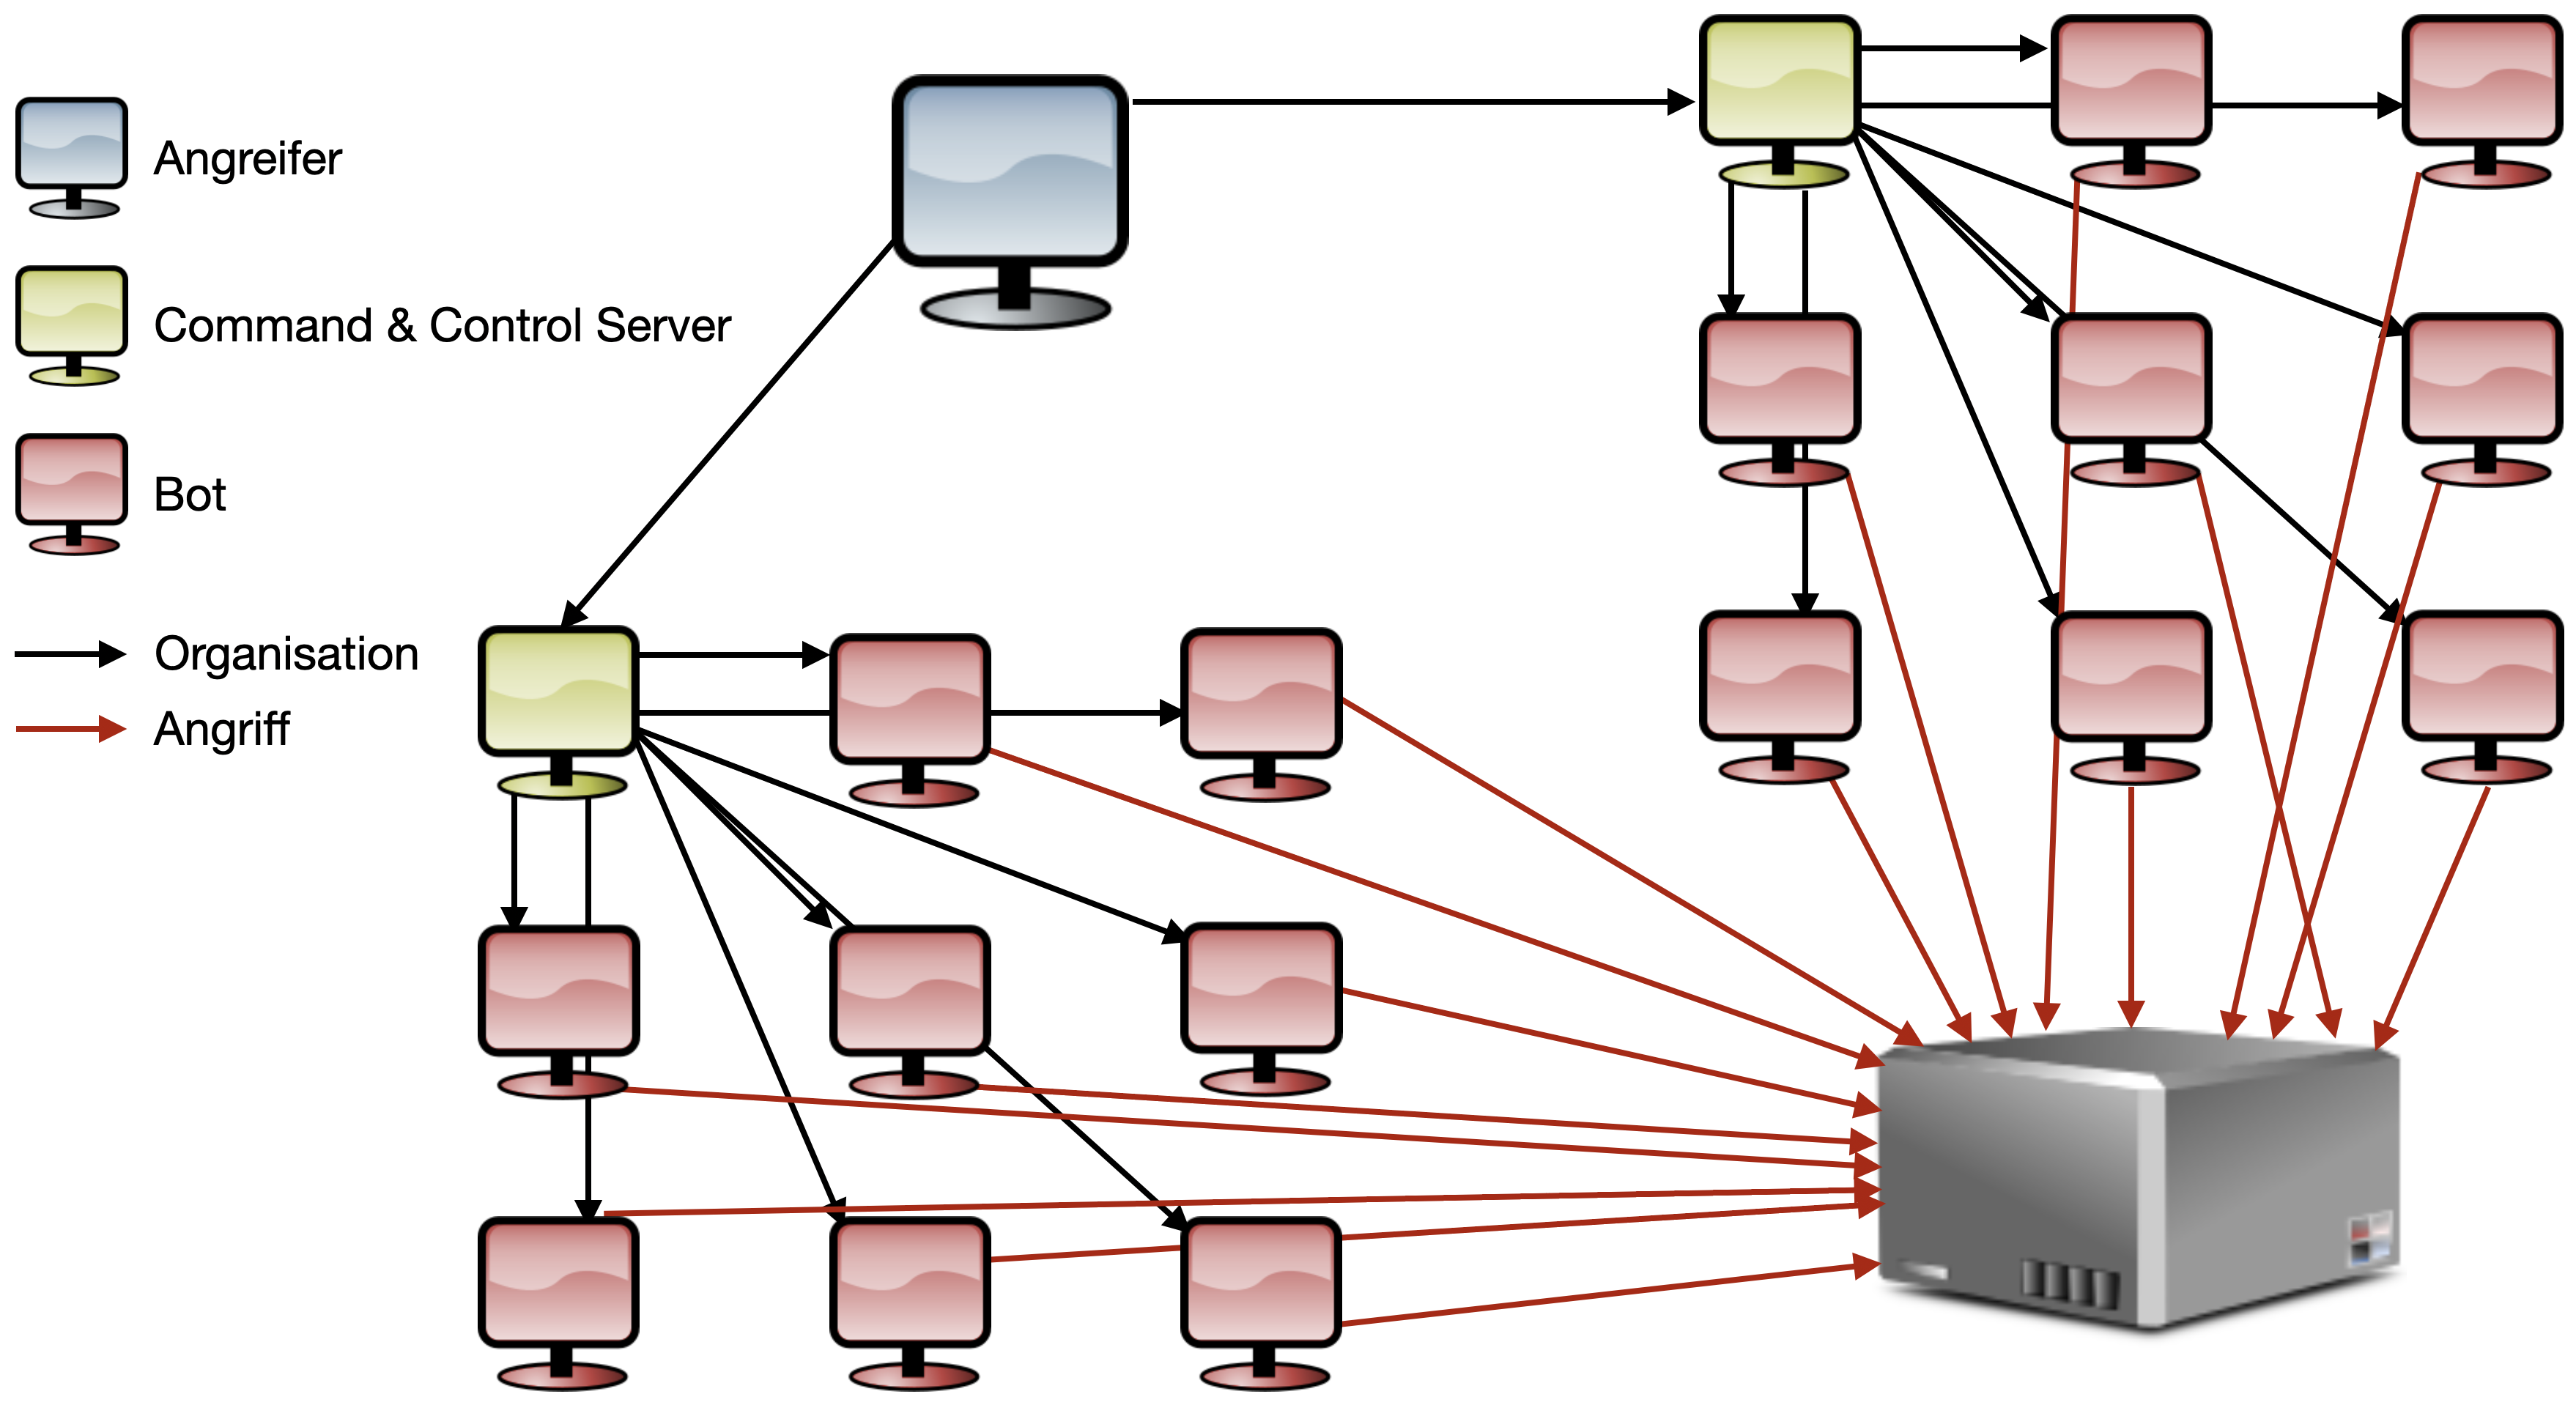
\includegraphics[width=\textwidth, center]{kapitel1/botnet}
		\caption[Schematischer Aufbau bei einem DDoS-Angriff mit einem Botnetz]{Schematischer Aufbau eines Botnetzes zur Durchführung eines DDoS-Angriffs}
		\label{img:botnet}
\end{figure}

\section{DDoS-Malware}

Eine weitere Möglichkeit, um einen DDoS-Angriff vorzubereiten ist das Schreiben einer DDoS-Malware. Eine solche Malware ist darauf ausgelegt sich erst als Wurm zu verbreiten und später zu einem vorher bestimmten Zeitpunkt den DDoS-Angriff zu starten.

Ein Beispiel für so einen Angriff ist Mydoom. Dieser Wurm hatte die Aufgabe auf infizierten Systemen eine Backdoor zu hinterlassen und einen DDoD Angriff gegen die SCO Group am 1.2.2004 zu starten. Zu diesem Zeitpunkt waren geschätzte 1.000.000 Computer mit dem Virus infiziert. Mydoom ist bis heute einer der massivsten DDoS-Angriffe und der sich am schnellsten verbreitende E-Mail Wurm.

\section{Angriffsziele}
\label{chap:kapitel4}

Führt ein Angreifer eine DDoS-Attacke durch, kann dies mehr, als nur ein Ziel haben. Im Folgenden sollen einige Ziele erklärt werden.

\subsection{Degradation of Service}

Bei dem Ziel Degradation of Service geht nicht darum ein gesamtes System oder einen Server komplett lahm zu legen, sondern nur darum, die Qualität des angegriffenen Servers zu reduzieren. Damit werden beim Angriff also nicht Ressourcen des Servers restlos aufgebraucht, aber ein bedeutenden Teil davon. Versucht nun ein Nutzer reguläre Anfragen an den Server zu schicken muss mit erhöhten Wartezeiten und eventuell mit fehlgeschlagenen Verbindungen gerechnet werden. Eine Degradation of Service ist vor allem auch dann ein vielversprechendes Ziel, wenn der Betreiber des angegriffenen Servers seine Ressourcen bei einem Anbieter nach Auslastung bezahlt. Durch erhöhte Auslastung beim Server während des Angriffs entstehen dann beträchtliche Mehrkosten beim Anbieter. Weiterhin gibt es den Vorteil, dass es schwer sein kann den Angriff von normalem erhöhtem Traffic zu unterscheiden.

\subsection{Denial of Service}

Hierbei geht es wirklich darum einen Server komplett außer Funktion zu bringen. Ein gutes Beispiel hierfür ist der Ping of Death. Mit diesem Angriff konnte bis vor einigen Jahren ein modifizierter Ping an Unix Systeme geschickt werden, der einen Systemabsturz zur Folge hatte. Damit war der Server von außen nicht mehr erreichbar und musste neu gestartet werden. Gerade für viel besuchte Websites, wie YouTube oder Netflix könnte so etwas sehr teuer werden, wenn der Fehler erst spät gefunden wird.

\subsection{Ablenkung}

Es kann auch möglich sein, dass DDoS Angriffe allein zur Ablenkung durchgeführt werden. Es ist gut möglich, dass ein Angreifer ein Ziel mit einer anderen Angriffsvariante verfolgt und gleichzeig einen DDoS Angriff auf einen anderen Server des gleichen Unternehmens durchführt. Dadurch, dass der DDoS Angriff Aufmerksamkeit und Personal an sich bindet hofft der Angreifer darauf, dass der eigentliche Angriff gar nicht erst entdeckt wird oder  weniger Personal dafür verfügbar ist etwas gegen eigentliche Bedrohung zu tun.

\subsection{Erpressung}

Ein weiteres Ziel kann eine Erpressung des Betreibers des Servers sein. Hierbei wird meist ein kleiner gestartet. Zeitgleich wird dem Betreiber des Servers eine Nachricht geschickt die mit einem wesentlich stärkeren Angriff droht und eine Geldsumme für das Abbrechen des Angriffs fordert. Diese Forderungen beziehen sich normalerweise auf Kryptowährungen wie Bitcoin, damit der Angreifer auch mit dem erhalten des Geldes anonym bleiben kann. Experten raten allerdings immer davon ab solchen Forderungen nachzugeben.
